\documentclass[thesis.tex]{subfiles}

\title{Estimating duration in the presence of misclassification}
\author{Joshua Blake}
\date{\today}

\begin{document}

\ifSubfilesClassLoaded{
  \setcounter{chapter}{1}
}

\chapter{SARS-CoV-2: biology and data} \label{biology-data}

SARS-CoV-2 is a beta coronavirus that emerged in late 2019.
It is closely related to previous coronaviruses that have caused outbreaks in humans, SARS-CoV and MERS-CoV.
\todo{Cite and check how SARS-CoV-2 is related to SARS-CoV and MERS-CoV, and other human coronaviruses.}

Coronaviruses are RNA\todo{spell out the acronym RNA} viruses.
RNA viruses use RNA, rather than DNA, as their genetic material.
\todo{why is being a RNA virus important?}

\section{Natural history of the disease} \label{biology-data:sec:natural-history}

\begin{figure}
  \centering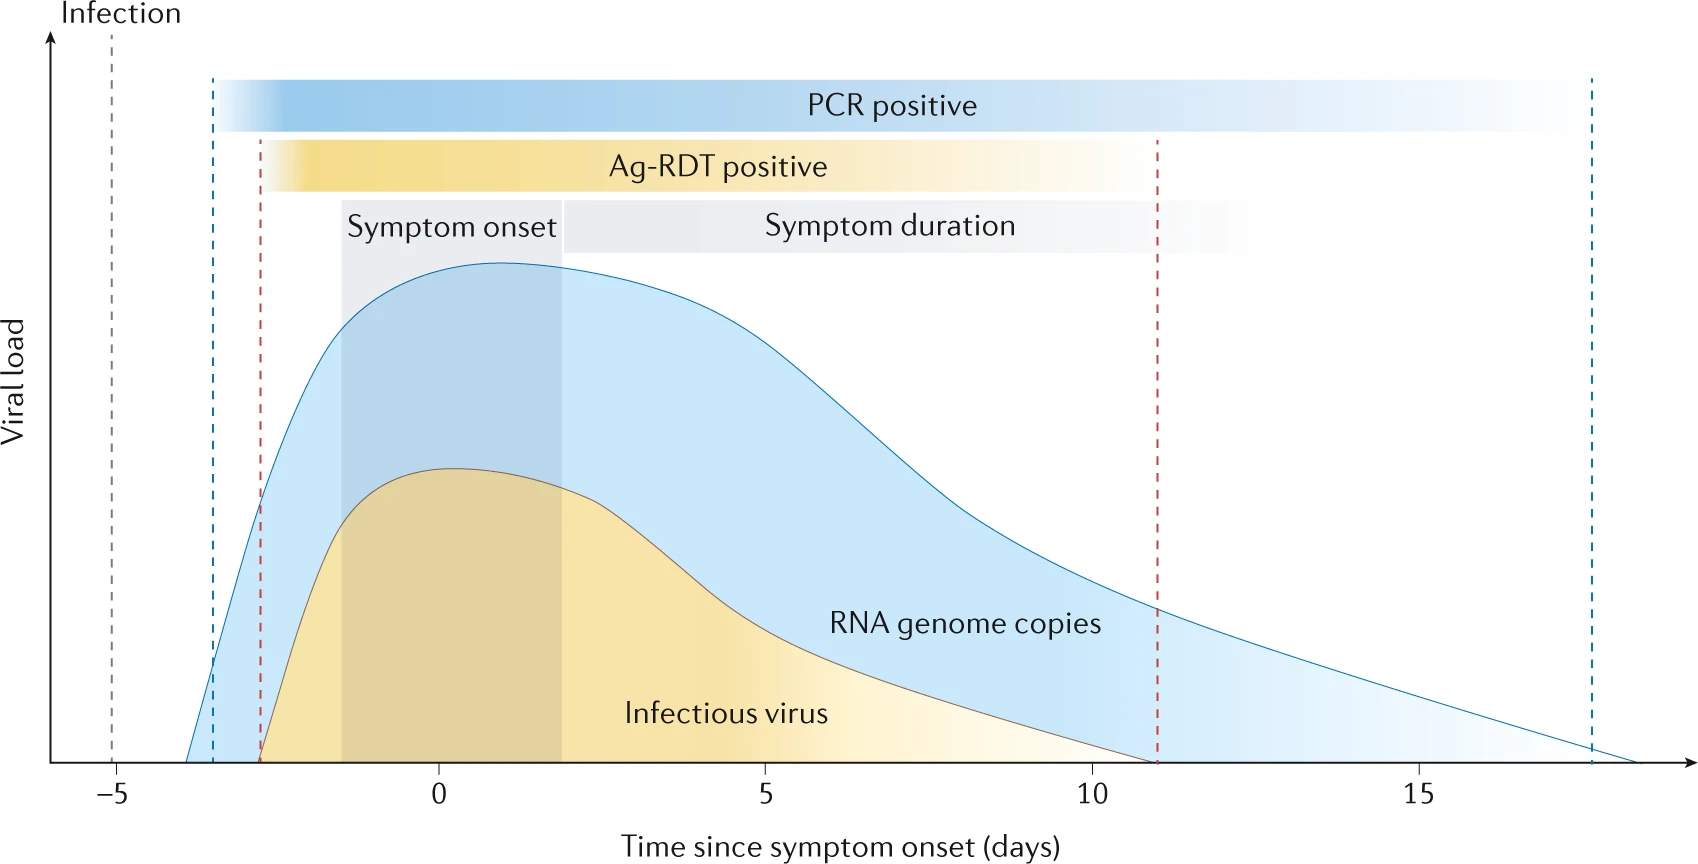
\includegraphics[width=\textwidth]{biology-data/natural-history}
  \caption[Natural history of SARS-CoV-2.]{Natural history of SARS-CoV-2. Reproduced from \textcite{puhachSARSCoV2} with permission.}
  \todo[inline]{Define the acronyms and terminology in the figure.}
  \label{biology-data:fig:natural-history}
\end{figure}

An individual infected with SARS-CoV-2 goes through several stages (see \cref{biology-data:fig:natural-history}).
\todo{Find citations for disease stages.}
First, they are exposed to the virus and become infected.
At this initial stage they are not infectious (cannot spread the disease to others), do not have symptoms, and will not test positive on a PCR test.
After a few days, they will start testing positive on a PCR test; this is normally prior to being infectious or having symptoms.
Next, the individual becomes infectious; normally, this occurs prior to symptom onset for those who experience symptoms.
Recovery from symptoms occurs after a few days, around individual is no longer infectious.
Finally, the individual will test negative on a PCR test.
\todo{Talk about PCR testing detecting RNA material even with no viable virus.}

The time for each of these stages depends on various features of host and virus characteristics.
In this thesis, I focus on pre-Alpha variants of SARS-CoV-2 in unvaccinated individuals.
The time from infection to infectiousness is known as the \emph{latent period} and is typically around\todo{cite latent period}.
The time from infection to experiencing symptoms is known as the \emph{incubation period} and is typically around\todo{cite incubation period}.
The latent period is undefined for asymptomatic individuals, around\todo{cite proportion asymptomatic} of those infected.

The above description gives three possible ways to define an individual who is infected with SARS-CoV-2: based on their PCR test result, whether they are infectious, or whether they are symptomatic.
In this thesis, I adopt a definition of infection based on PCR test results.
This is because it coincides with the data collected on the studies I use (see \cref{biology-data:sec:studies}).

\todo[inline]{Add something about viral load being the process underlying these processes.}

% Possible summaries
% \begin{enumerate}
%   \item \url{https://www.nature.com/articles/s41579-022-00822-w/figures/2}
%   \item \url{https://www.nature.com/articles/s41576-021-00360-w/figures/1}
%   \item \url{https://academic.oup.com/view-large/figure/305617142/ciaa1442_fig2.jpg}
% \end{enumerate}

\section{PCR testing} \label{biology-data:sec:PCR}

\todo[inline]{Consider finding or making a figure to explain PCR testing.}

PCR testing consists of a series of cycles, each cycle containing a three-step process.
PCR testing is used to detect the prence of a specific sequence of DNA in a sample.
However, SARS-CoV-2 is an RNA virus and hence the first step is to convert the RNA to DNA.
This step is known as reverse transcription, with the whole process being known as reverse-transcription polymerase chain reaction (RT-PCR).

Reverse transcription is the process of converting RNA to DNA.
In reverse transcription, a naturally-occurring enzyme known as reverse transcriptase generates the complementary DNA (cDNA) from the RNA template.
\todo{Maybe explain what it means for RNA to have cDNA and what a template is.}
The cDNA can then be used in the standard PCR process.

The first step of the PCR cycle is \emph{denaturation}.
In denaturation, the DNA is heated to separate the two strands of DNA.
The second step is \emph{annealing}.
In annealing, the temperature is lowered to allow primers to bind to the DNA.
Primers are short sequences of DNA that are complementary to the DNA sequence of interest.
By choosing the primer that matches the cDNA sequence that we want to detect the PCR test can be made specific to the virus of interest.
The final step is \emph{extension}.
In extension, the temperature is raised to allow the enzyme DNA polymerase to extend the primers and hence replicate the DNA sequence of interest.
\todo{Check all these temperatures and maybe remove specifics?}

Over the course of the cycle, the amount of DNA doubles (although there is some stochastic variation).
Therefore, the number of DNA copies at the end of each cycle increases geometrically.
Once enough DNA has been produced, the DNA can be detected by various methods.
The number of cycles required to reach detection is known as the \emph{cycle threshold} (Ct) value.

The Ct value increases linearly as the logarithm of the amount of RNA present in the original sample.
That is, smaller Ct values correspond to larger amounts of RNA in the original sample.
If there is more RNA present, more cDNA is created, and hence fewer cycles are required to reach detection.
The logarithm is because the process is geometric, and hence the number of DNA copies increases linearly on the log-scale.
\todo{Clearer explanation}

Like any diagnostic test, PCR tests are not perfect.
False positives and false negatives can occur.
The \emph{specificity} of a test is the probability of a negative test result given that the individual is not infected.
The \emph{sensitivity} of a test is the probability of a positive test result given that the individual is infected.

False positives are very rare for PCR tests.
In summer 2020, the CIS performed X PCR tests and found only Y positives, lower-bounding the test positivity at.
\todo{Insert actual numbers of CIS bounding specificity.}
Due to the very high specificity, I ignore false positives in this thesis.

False negatives are more common.
Early estimates of the sensitivity of PCR tests were around X\%; I produce estimates in \cref{E-ATACCC}.
False negatives could occur for a variety of reasons, most commonly that an individual swabs themselves poorly and hence the concentration of virus on the swab is too low to be detected by the PCR process.
Plausibly, a variety of other reasons could also lead to a false negative such as logistical issues or mislabelling of samples.
\todo{Cite reasons false negative results occur.}

The minimum amount of virus required to be detected by a PCR test is known as the \emph{limit of detection}.
\todo{Cite limit of detection and explain a bit more about it.}

Viral loads are infrequently measured exactly.
The most common form of data obtained is cycle threshold (Ct) values from real-time quantitative  reverse-transcriptase polymerase chain reaction (PCR) tests.
The Ct value is proportional to the negative log of the viral load which is convenient when modelling log viral load as a piecewise linear function, since Ct values themselves are piecewise linear under this assumption.
When a host's viral load is too low (below the limit of detection of the PCR test), no Ct value is available and hence viral load can be considered censored at the limit of detection.
The relationship between Ct and viral load is noisy and can vary based on many factors including quality of swab obtained, primers used (even between batches), and the PCR system set-up~\autocites{dahdouhCt,hanRTPCR}.

\todo[inline]{Include the idea of being "detectable"? Check if/where/how I've used this concept in current version of text.}

\section{Studies used in this thesis} \label{biology-data:sec:studies}

\subsection{Assessment of Transmission and Contagiousness of COVID-19 in Contacts}

\subsection{Coronavirus (COVID-19) Infection Survey} \label{intro:sec:cis}

The CIS (Coronavirus (COVID-19) Infection Survey) continually enrols individuals and tests them on an ongoing basis, following a specified testing protocol.
The protocol specifies that the initial five tests are spaced every 7 days, then the spacing is every 28 days.
However, real-world considerations often lead to variations in test times and missed tests.

The CIS (Coronavirus Infection Survey) is a longitudinal study on a representative sample of households.
Households are invited to the study from databases held by the ONS.
The number invited was to satisfy various target number of individuals swabbing per fortnight.
Within a selected household, all individuals aged 2 and over were invited to participate.
Once invited, an enrolment swab would be taken followed by 4 further weekly swabs (giving a total of 5 swabs on days 0, 7, 14, 21, 28 relative to enrolment) after which monthly swabs are taken.
A full description of the study can be found in \textcite[][supplementary materials]{pouwelsCommunity} or the study protocol~\autocite{cisProtocol}.

During the period we consider, the total cohort size expands due to the continuous recruitment into the study.
Following this, the number then decreases and stabilises as those recruited to meet the October target transition from weekly onto monthly testing.

\todo[inline]{Add some descriptive figures e.g. those in \url{~/COVID/ons-incidence/duration_estimation/reproducible-sims/reports/simulation-studies.pdf}}

\begin{figure}
  \centering 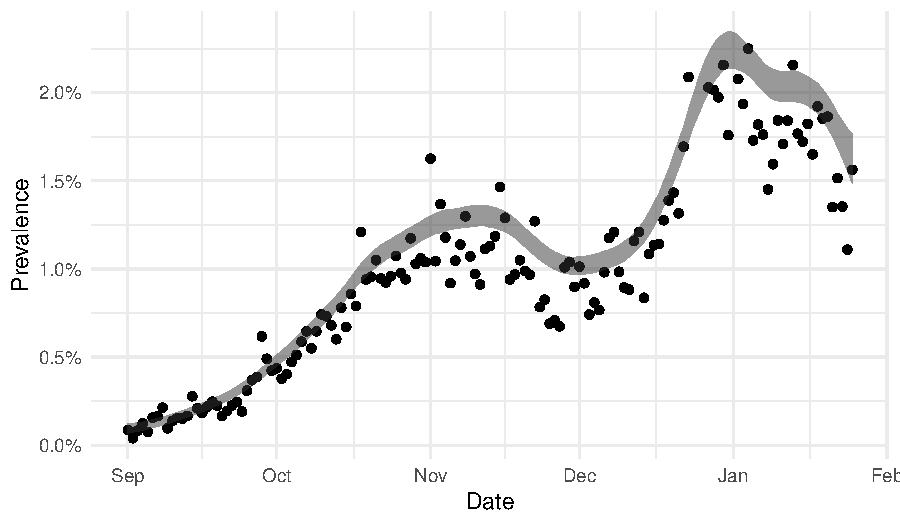
\includegraphics[width=\textwidth]{biology-data/CIS-positivity}
  \caption[CIS prevalence]{%
    CIS prevalence in the period considered in this thesis (Sep 2020 until Jan 2021).
    Dots show raw proportion of non-void tests that are positive on each day (days with fewer than 100 tests excluded for readability).
    Ribbon shows modelled 95\% CrI for the prevalence, corrected for non-response bias and smoothed over time (using the methodology described in \cref{E-backcalc:sec:methods}).
    The correction tends to increase the estimated prevalence because underrepresented groups tend to have higher prevalence.
  }
\end{figure}
\begin{figure}
  \centering 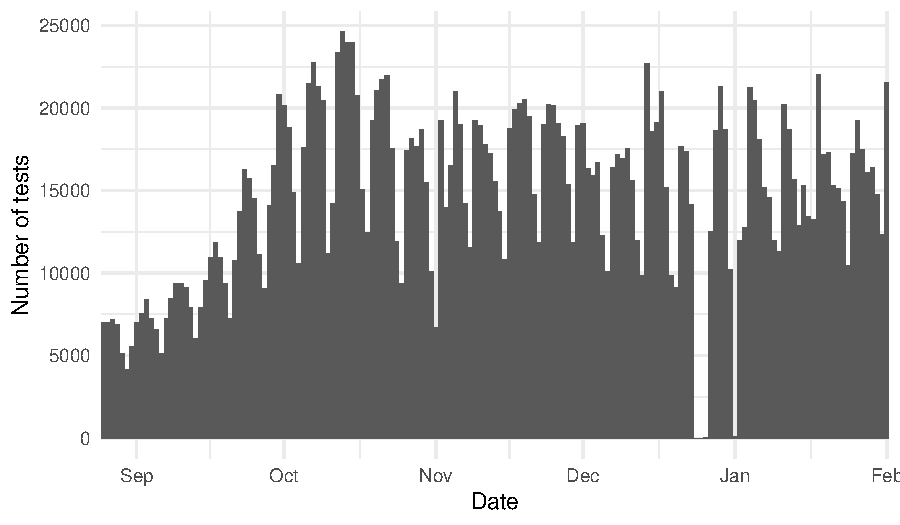
\includegraphics[width=\textwidth]{biology-data/CIS-num-tests}
  \caption[Number of CIS tests]{%
    Daily number of CIS tests conducted in the period considered in this thesis (Sep 2020 until Jan 2021).
  }
\end{figure}

Consider the CIS data.
It consists of a series of tests on the same individuals (longitudinal data), where some individuals have a series of positive tests.

\subsubsection{Episodes}

\emph{Explain definition in ``SARS-CoV-2 reinfection definition'' from \textcite{weiRisk}.}

\emph{Intermittent negatives} are the clearest example of a false negative.
An intermittent negative is when an individual tests negative but tested positive previously and subsequently.
Intermittent negatives are stripped out when creating the dataset used for all duration analyses in this chapter, but demonstrate that false negatives do occur.

% Whether a future positive is part of the same episode of a reinfection is not always trivial; I rely on a process developed previously by Sarah Walker, see \cref{E-episode-def}.
However, up until the emergence of the Omicron variant, reinfections are rare, especially in a short time frame, and hence the tricky cases are rare until this time (late 2021).


\ifSubfilesClassLoaded{
  \listoftodos
}{}

\end{document}